\documentclass[tikz]{standalone}
\usepackage{frenchmath}

\begin{document}
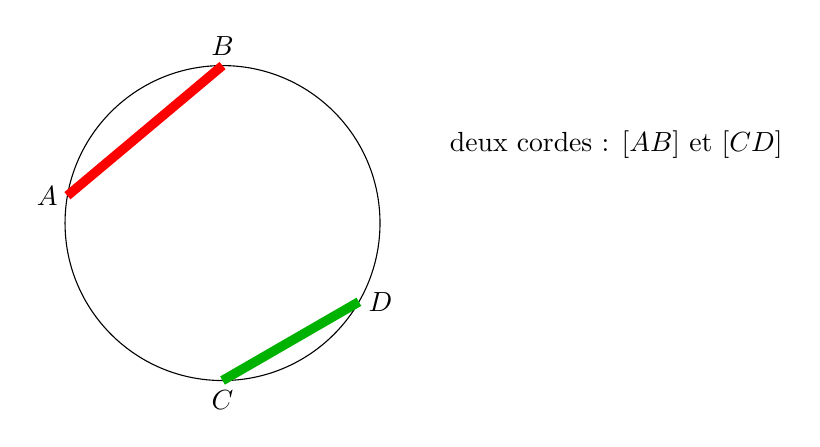
\begin{tikzpicture}
    \draw (0,0) circle (2);
    \coordinate (A) at ({2*cos(170)},{2*sin(170});
    \coordinate (B) at ({2*cos(90)},{2*sin(90});
    \coordinate (C) at ({2*cos(270)},{2*sin(270});
    \coordinate (D) at ({2*cos(330)},{2*sin(330});
    \draw[line width=1.2mm,red] (B) -- (A);
    \draw[line width=1.2mm,green!70!black] (C) -- (D);
    \foreach \p/\x in {A/left,B/above,C/below,D/right} {
        \node[\x] at (\p) {$\p$};
    }
    \node at (5,1) {deux cordes : $[AB]$ et $[CD]$};
\end{tikzpicture}
\end{document}